\documentclass[conference]{IEEEtran}
\usepackage[top=3cm, bottom=2cm, left=2cm, right=2cm, columnsep=20pt]{geometry}
\usepackage{pdfpages}
\usepackage{graphicx}
\usepackage{etoolbox}
\apptocmd{\sloppy}{\hbadness 10000\relax}{}{}
% \usepackage[numbers]{natbib}
\usepackage[T1]{fontenc}
\usepackage{ragged2e}
\usepackage[french]{babel}
\usepackage{listings}
\usepackage{color}
\usepackage{soul}
\usepackage[utf8]{inputenc}
\usepackage[export]{adjustbox}
\usepackage{caption}
\usepackage{amsmath}
\usepackage{amssymb}
\usepackage{float}
\usepackage{csquotes}
\usepackage{fancyhdr}
\usepackage{wallpaper}
\usepackage{siunitx}
\usepackage[indent]{parskip}
\usepackage{textcomp}
\usepackage{gensymb}
\usepackage{multirow}
\usepackage[hidelinks]{hyperref}
\usepackage{abstract}
\usepackage{subcaption}
\usepackage{tabularx}

% \renewcommand{\abstractnamefont}{\normalfont\bfseries}
% \renewcommand{\abstracttextfont}{\normalfont\itshape}
\usepackage{titlesec}
% \titleformat{\section}{\large\bfseries}{\thesection}{1em}{}
% \titleformat{\subsection}{\normalsize\bfseries}{\thesubsection}{1em}{}
% \titleformat{\subsubsection}{\normalsize\bfseries}{\thesubsubsection}{1em}{}

\usepackage{xcolor}
\definecolor{codegreen}{rgb}{0,0.6,0}
\definecolor{codegray}{rgb}{0.5,0.5,0.5}
\definecolor{codepurple}{rgb}{0.58,0,0.82}
\definecolor{backcolour}{rgb}{0.95,0.95,0.92}
\lstdefinestyle{mystyle}{
    backgroundcolor=\color{backcolour},   
    commentstyle=\color{codegreen},
    keywordstyle=\color{magenta},
    numberstyle=\tiny\color{codegray},
    stringstyle=\color{codepurple},
    basicstyle=\ttfamily\footnotesize,
    breakatwhitespace=false,         
    breaklines=true,                 
    captionpos=b,                    
    keepspaces=true,                 
    numbers=left,                    
    numbersep=5pt,                  
    showspaces=false,                
    showstringspaces=false,
    showtabs=false,                  
    tabsize=2
}
\lstset{style=mystyle}

\usepackage[most]{tcolorbox}
\newtcolorbox{note}[1][]{
  enhanced jigsaw,
  borderline west={2pt}{0pt}{black},
  sharp corners,
  boxrule=0pt, 
  fonttitle={\large\bfseries},
  coltitle={black},
  title={Note:\ },
  attach title to upper,
  #1
}

%----------------------------------------------------

\setlength{\parindent}{0pt}
\DeclareCaptionLabelFormat{mycaptionlabel}{#1 #2}
\captionsetup[figure]{labelsep=colon}
\captionsetup{labelformat=mycaptionlabel}
\captionsetup[figure]{name={Figure }}
\captionsetup[table]{name=Tableau}
\newcolumntype{Y}[1]{>{\Centering\hspace{0pt}\hsize=#1\hsize}X}
\newcommand{\inlinecode}{\normalfont\texttt}
\usepackage{enumitem}
\setlist[itemize]{label=\textbullet}

\begin{document}

%----------------------------------------------------
\title{Écran tactile acoustique\\
\large Travail préparatoire \\
PHS3910 -- Techniques expérimentales et instrumentation\\ 
Équipe L3}

\author{\IEEEauthorblockN{Émile Guertin-Picard}
\IEEEauthorblockA{2208363}
\and
\IEEEauthorblockN{Maxime Rouillon}
\IEEEauthorblockA{2213291}
\and
\IEEEauthorblockN{Marie-Lou Dessureault}
\IEEEauthorblockA{2211129}
\and
\IEEEauthorblockN{Philippine Beaubois}
\IEEEauthorblockA{2211153}
}

\maketitle

\textit{\textbf{Résumé} -- Dans l'optique de développer un piano tactile fonctionnel,
des simulations ont été effectuées sur MatLab à l'aide du module k-Wave afin d'optimiser
certains paramètres (forme, matériau et position du capteur) du prototype à conceptualiser. 
Il a été conclut qu'une plaque asymétrique en plexiglas, ayant 
un capteur placé proche d'un de ses côtés, serait idéale pour maximiser le contraste et minimiser la résolution 
lors de la détection de signaux tactiles.}


\section{Introduction}
Dans le cadre du cours PHS3910, l'équipe est mandatée de conceptualiser
un piano tactile à l'aide du principe de retournement temporel. Avant
de développer le produit final, il faut premièrement simuler le fonctionnement 
du piano à l'aide de l'outil k-Wave, afin de déterminer les caractéristiques qui 
optimiseront sa performance. En variant la forme, le matériau de 
la plaque ainsi que la position du capteur directement dans la simulation,
une solution complète préliminaire peut être établie. Le choix de la solution finale est
principalement basée sur les concepts de résolution et de contraste.

Les choix retenus suite aux tests de simulation sont les suivants: une plaque
asymétrique avec trous, en plexiglas, avec un capteur situé proche d'un de ses côtés.
Le rapport ci-présent détaillera la méthodologie utilisée afin d'obtenir 
une étude statistique de la résolution et du contraste en fonction des
caractéristiques du piano, présentera les valeurs résultantes et leurs incertitudes 
respectives, et discutera des éléments pouvant être déduits de ceux-ci et implémentés 
dans la conception.

\section{Méthodes \label{methodes}}
%Garder en tête qu'on veut ''On vous demande de déterminer et de 
%faire une étude systémique et rigoureuse des paramètres
%principaux à optimiser. ''

%''piano tactile le plus près possible d’un piano acoustique''

%Méthodes : Transformer cette question dans un langage mathématique, 
%décrire les méthodes de simulations
Étant donné que le problème à considérer est de trouver les paramètres 
optimaux à l'aide d'une simulation, les méthodes de simulations sont décrites
en fonction des étapes importantes du programme MatLab utilisant le module K-Wave. % MatLab -> MATLAB (oui c'est un tit détail je sais)
Les formes des plaques considérées ont été choisies pour avoir un éventail de 
géométries (carré, forme asymétrique, avec et sans trous). Du plexiglas et de 
l'aluminium ont été testés pour déterminer l'impact du milieu sur le contraste et la résolution. 
Les simulations se limitent à ces matériaux car ce sont ceux à disposition 
pour la construction du piano.

Pour étudier l'impact du matériau, de la géométrie et de la position du capteur
individuellement, deux paramètres ont été fixés avant de faire varier le troisième. 
L'interdépendance entre les paramètres a été considérée comme négligeable dans 
les modèles.

Le signal \textit{$S_{ij}$(t)} obtenu à un récepteur à un point \textit{$P_i$} a été
modélisé comme la réponse impulsionnelle de la configuration (géométrie et matériau) 
à une impulsion d'une source à un endroit \textit{$S_j$}. 
L'impulsion a été modélisée par un delta de dirac \textit{$\delta$} qui est 
l'identité du produit de convolution. On a donc
%
\[S_{ij}(t)=(h_{P_iS_j} * \delta)(t)=h_{P_iS_j}(t).\]
%
Le signal obtenu était de la forme d'une onde se propageant dans le matériau. Or, 
cette équation admettait également comme solution $h_{P_jS_i}(-t)$. Ce retournement
temporel revenait à parcourir le temps de façon opposée, ce qui impliquait également 
d'intervertir les rôles de récepteur et d'émetteur. 
%
%Plus d'explications de MATHS ici (Voir cahier rouge)
% Pour chaque configuration, au lieu de simuler un émetteur pour un grand nombre de 
% positions, il a plutôt été convenu d'effectuer la simulation d'un seul emplacement 
% et d'utiliser le principe du retournement temporel.  
% Ainsi, un seul impact a eu besoin d'être simulé à un endroit arbitraire en évaluant 
% le signal reçu à une multitude de récepteurs distribués sur la plaque. 
% À la suite du retournement temporel, les positions \textit{i} et \textit{j} 
% sont intervertis. 
Pour chaque source, le signal au récepteur \textit{$S_{ij}$} est devenu:
\[S_{ij}(t)=h_{P_jS_i}(-t).\]
Une fois la réponse impulsionnelle obtenue pour tous les emplacements désirés 
sur la plaque, les décalages entre les signaux ont été retirés en gardant seulement 
une fenêtre de la réponse impulsionnelle.
Les signaux inversés et recadrés ont été stockés pour pouvoir s'y 
référer lors du calcul de la corrélation \textit{$C_{ij}$} entre les réponses impulsionnelles de la 
source et de l'émetteur. 
Cette corrélation a été donnée par:
\[C_{ij}(t)=h_{P_iS_j}(t)*h_{P_jS_i}(-t).\]
%
%Corrélation
Une bande d'intérêt sur la plaque a été choisie pour réduire le temps de calcul. 
Pour chaque point de la bande, la corrélation entre son signal et celui 
des autres points a été calculée. 
Un graphique 2D de la corrélation en fonction de la position sur la bande a été fait. 
Pour effectuer une analyse statistique de la résolution et du contraste, il a fallu 
faire correspondre une courbe gaussienne sur chaque graphique 2D obtenu. 
La largeur à mi-hauteur de la gaussienne a pu déterminer la résolution alors que la 
différence entre le maximum de la courbe et le niveau du bruit a pu déterminer le contraste.
Les valeurs finales et leur incertitude respective découlent des impulsions choisies 
pour l'analyse statistique; la moyenne et l'écart-type pour chaque variable sont calculées.


\section{Résultats}
Les géométries testées lors des simulations sont exemplifiées dans la figure \ref{fig:fig}. La ligne rouge
sur chaque géométrie définie la bande d'intérêt des sources; elle est positionnée
sur l'axe où les touches du piano seraient placées pour un prototype.
\begin{figure}[H]
  \begin{subfigure}{.155\textwidth}
    \centering
    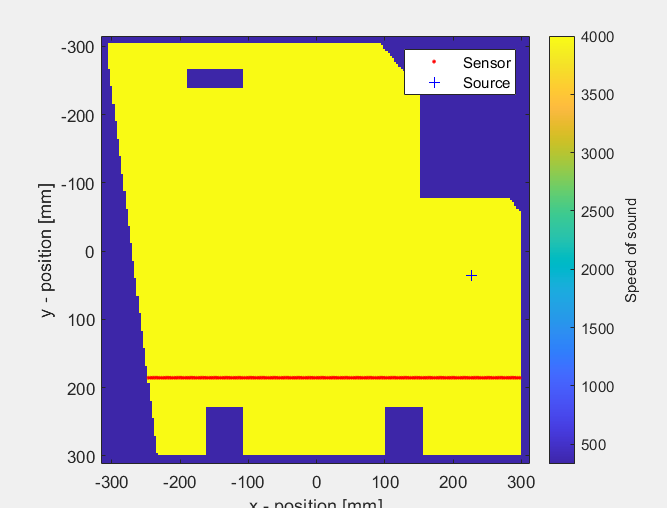
\includegraphics[width=.95\linewidth]{forme1.png}
    \caption{}
    \label{fig:sfig1}
  \end{subfigure}%
  \begin{subfigure}{.155\textwidth}
    \centering
    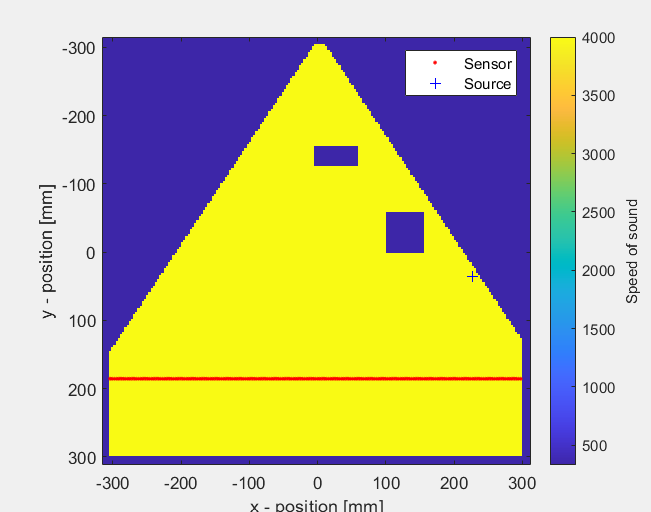
\includegraphics[width=.95\linewidth]{forme2.png}
    \caption{}
    \label{fig:sfig2}
  \end{subfigure}
  \begin{subfigure}{.155\textwidth}
    \centering
    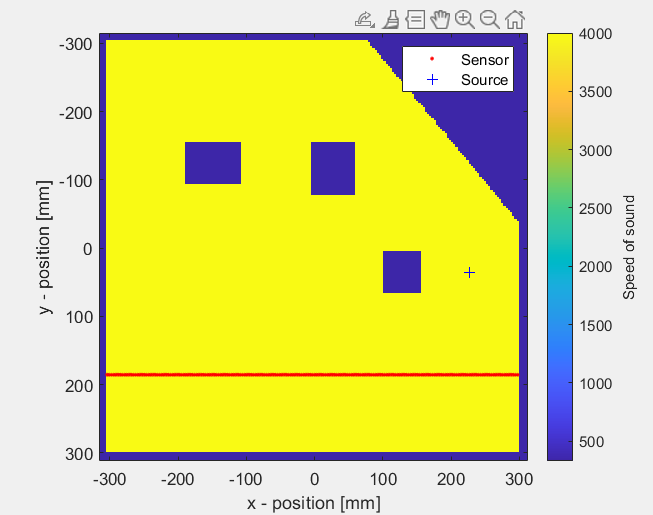
\includegraphics[width=.95\linewidth]{forme3.png}
    \caption{}
    \label{fig:sfig3}
  \end{subfigure}
  \begin{subfigure}{.155\textwidth}
    \centering
    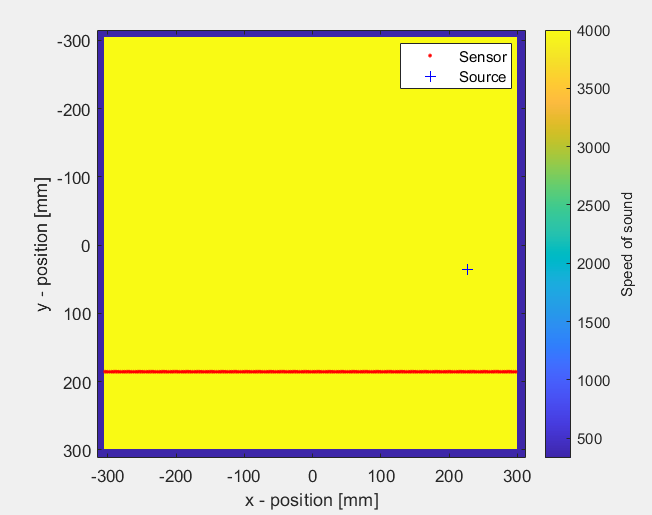
\includegraphics[width=.95\linewidth]{forme4.png}
    \caption{}
    \label{fig:sfig4}
  \end{subfigure}
  \begin{subfigure}{.155\textwidth}
    \centering
    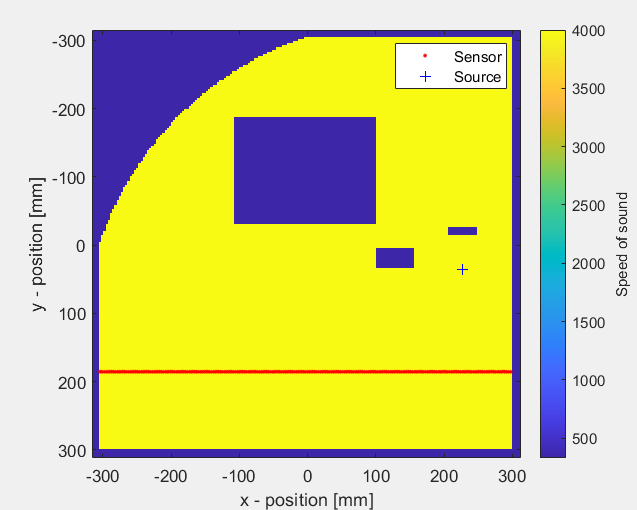
\includegraphics[width=.95\linewidth]{forme5.png}
    \caption{}
    \label{fig:sfig5}
  \end{subfigure}
  \begin{subfigure}{.155\textwidth}
    \centering
    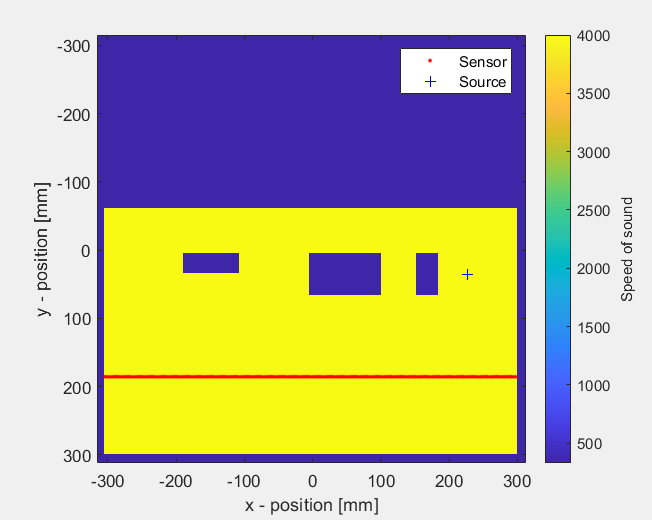
\includegraphics[width=.95\linewidth]{forme6.png}
    \caption{}
    \label{fig:sfig6}
  \end{subfigure}
  \caption{Géométries considérées pour les simulations}
  \label{fig:fig}
\end{figure}
Pour chaque géométrie, trois positions arbitraires pour le capteur ont été choisies,
chacune étant associée à un ensemble de coordonnées. À titre de référence, la position $(0,0)$ se situe 
en haut à gauche des grilles des figures \ref{fig:sfig1} à \ref{fig:sfig6}.  

\begin{table}[H]
\begin{tabularx}{\columnwidth}{@{} Y{1.00} Y{0.75} Y{1.00} Y{1.35} Y{0.87} @{}}
  \hline
  Matériau&Géométrie&Position du capteur&Contraste&Résolution\\
  \hline
  \multicolumn{5}{c}{Valeurs de contraste les plus élevées}\\
  \hline
  Plexiglas&(a)& 100, 100& $0.83 \pm 0.01$ & $8 \pm 1$ \\
  Plexiglas&(c)& 20, 100& $0.825 \pm 0.008$ & $7.7 \pm 0.2$ \\
  Plexiglas&(a)& 50, 100& $0.823 \pm 0.006$ & $8.4 \pm 0.8$ \\
  \hline
  \multicolumn{5}{c}{Valeurs de contraste les plus faibles}\\
  \hline
  Aluminium&(b)& 25, 100& $0.75 \pm 0.02$ & $15 \pm 2$ \\
  Aluminium&(e)& 110, 170& $0.76 \pm 0.01$ & $6.6 \pm 0.5$ \\
  Aluminium&(f)& 100, 30& $0.768 \pm 0.006$ & $12 \pm 2$ \\
  \hline
  \multicolumn{5}{c}{Valeurs de résolution les plus élevées}\\
  \hline
  Aluminium&(e)& 110, 100& $0.80 \pm 0.01$ & $15 \pm 2$ \\
  Aluminium&(b)& 25, 100& $0.75 \pm 0.02$ & $15 \pm 2$ \\
  Aluminium&(a)& 100, 100& $0.82 \pm 0.02$ & $15 \pm 4$ \\
  \hline
  \multicolumn{5}{c}{Valeurs de résolution les plus faibles}\\
  \hline
  Plexiglas&(e)& 30, 100& $0.803 \pm 0.006$ & $8 \pm 1$ \\
  Plexiglas&(c)& 20, 100& $0.825 \pm 0.008$ & $7.7 \pm 0.2$ \\
  Plexiglas&(a)& 50, 100& $0.823 \pm 0.006$ & $8.4 \pm 0.8$ \\
  \hline
\end{tabularx}
\caption{Résumé des résultats des simulations}
\label{tableau_resultats}
\end{table}
En guise de résumé, les cas ayant les valeurs de contraste et de résolution les plus faibles et les plus élevées
sont présentés dans le tableau \ref{tableau_resultats}. Les valeurs de contraste et de 
résolution correspondent chacune à la moyenne de l'ensemble de données, et leur incertitude 
correspond à l'écart-type.




\section{Discussion}
Ayant obtenu un fit 2D gaussien, il est possible d'analyser et de comparer les variables pertinentes, 
le contraste et la résolution, selon différents paramètres physiques qui ont été élaborés dans la section \ref{}.
Le graphique \ref{} offre un échantillon des résultats obtenus pour une plaque carrée, sans trous et 
en bois. En ayant utilisé le retournement temporel, la durée de simulation a pu être réduite, ce qui a 
permis d'obtenir des réponses temporelles pour un nombre d'échantillons considérablement plus grand. 
Cette décision a permis d'améliorer la définition des fits gaussiens. Six échantillons ont été choisis au
hasard parmi les deux bandes considérées, offrant un poids statistique aux résultats assez important.

En observant le graphique \ref{}, on peut noter que l'emplacement de la source du signal
correspond à une corrélation de 1. Ceci s'explique facilement par le fait que le signal choisi au
hasard comme source et le signal de référence sont les mêmes (le choix de réutiliser le signal a été fait encore
une fois pour réduire le temps de compilation). La courbe gaussienne a une correspondance quasi parfaite pour les données
proches du maximum du pic, mais réduit en terme d'exactitude pour les données au niveau de la base
de la gaussienne.

Les résultats obtenus avec cette simulation permettent d'avoir un aperçu quant-aux
résultats possibles des simulations de d'autres paramètres. Le cas le plus favorable suite à 
un plus grand nombre de simulations serait d'avoir une résolution faible
et un contraste important. En évaluant l'allure de la courbe pour le cas ci-présent, on peut estimer
qu'il serait souhaitable de trouver des paramètres offrant un contraste plus grand que ceux évalués ici.
La résolution, quant-à-elle, semble déjà suffisament bonne. Évidemment, il est difficile d'arriver à une 
conclusion pertinente sans d'autres éléments de comparaison.



\clearpage

% \bibliographystyle{unsrtnat}
% \bibliography{My_Library}

\end{document}
